To provide a better understanding of the stock and flow model, the following section will explain the equations of some of the most important variables, which influence waste sorting behavior and ultimately the material recycling percentage. 

\section{Change in Frequency \& Frequency of Waste Collection}

\begin{figure}[H]
\centering
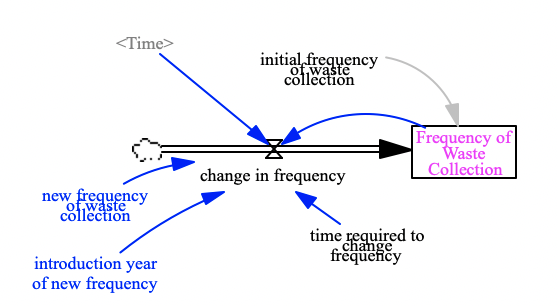
\includegraphics [scale=0.34,angle=360]{figures/frequency.png}
\caption{Change in Frequency \& Frequency of Waste Collection}
\label{fig:frequency}
\end{figure}	

\indent \newline
Change in frequency is modeled as an inflow and measures change in frequency over a period of time. The equation in the inflow "change in frequency" states that if time is less than the introduction of new frequency, then the value of change in frequency will be 0. If the introduction year of new frequency is greater than or equal to time, then the model computes the change in frequency per year (new frequency of waste collection- frequency of waste collection)/time required to change frequency. The frequency of waste collection is formulated as a stock and represents the frequency of waste collection at a specific time. 

\section{Complexity of Waste Management System}

\begin{figure}[H]
\centering
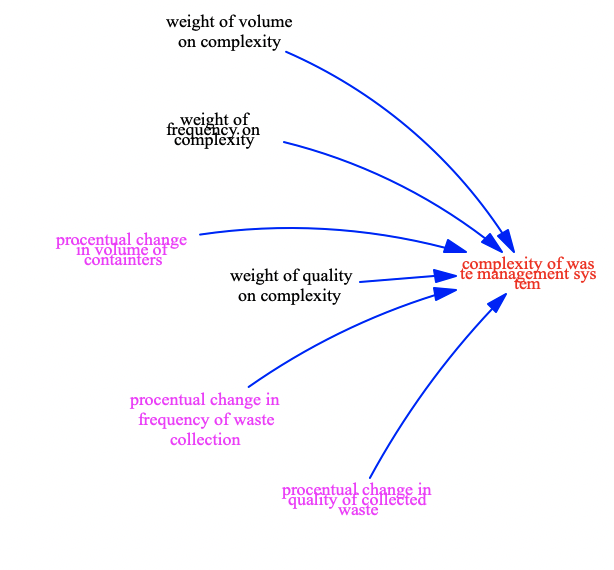
\includegraphics [scale=0.34,angle=360]{figures/complexityeq.png}
\caption{Complexity of Waste Management System}
\label{fig:complexityeq}
\end{figure}

\indent \newline
The variable "Complexity of waste management system" is a weighted average of three exogenous "weight" variables and their related three endogenous variables. The exogenous variables are weighted differently, which is based on the variable's impact on complexity of waste management system. If there is an increase in volume or frequency, the complexity decreases. This is due to  waste containers not overflowing with waste. When quality increases, the complexity increases since there are additional containers that complicate waste sorting. 

\section{Waste Sorting Behavior}

\subsection{Potential Waste Sorting Behavior}

\begin{figure}[H]
\centering
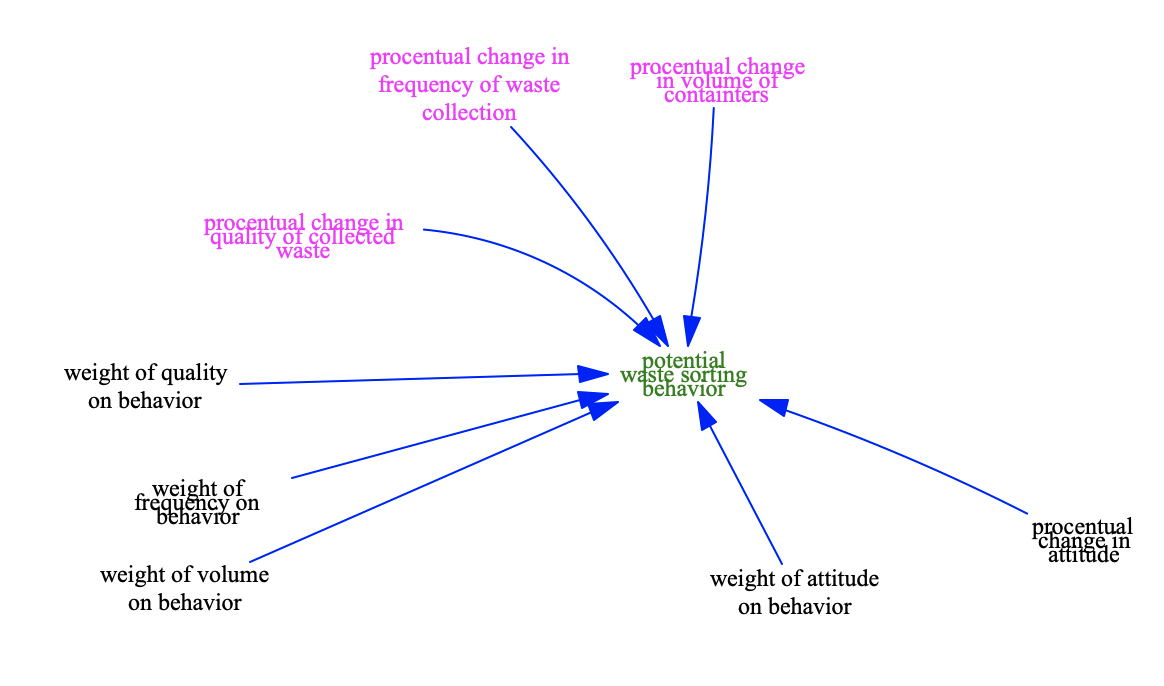
\includegraphics [scale=0.26,angle=360]{figures/potentialbehaviour.png}
\caption{Potential Waste Sorting Behaviour}
\label{fig:potentialbehaviour}
\end{figure}

\indent \newline
The endogenous variable "potential waste sorting behavior" computes the level of the potential sorting behavior. The equation shows that an increase in the volume of the rest waste containers decreases potential waste sorting behavior. A larger volume makes it easier for the citizens to throw everything in one container. An increase in quality and attitude  have a positive effect on potential waste sorting behavior. Additionally the equation states that an increase in the frequency of waste collection will have a positive effect on potential waste sorting behavior. The reason for this is that an increase in frequency will make it less likely that the waste containers will overflow. On the other hand, if the rest waste containers are full, the citizens will most likely throw the waste in the wrong container or just leave the waste next to the containers. 

\subsection{Change in Waste Sorting Behaviour}

\begin{figure}[H]
\centering
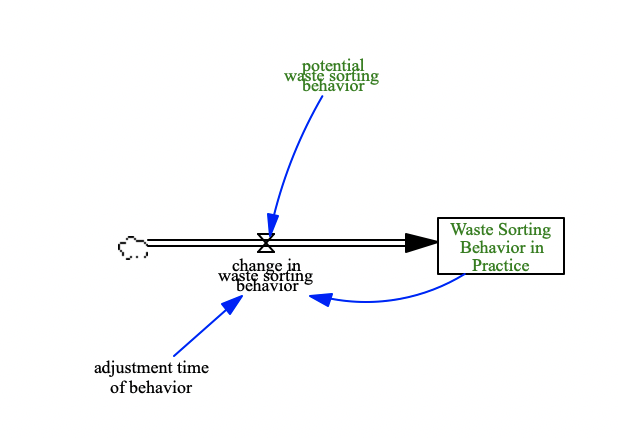
\includegraphics [scale=0.34,angle=360]{figures/changebehaviour.png}
\caption{Change in Waste Sorting Behavior \& Waste Sorting Behavior in Practice}
\label{fig:changebehaviour}
\end{figure}

\indent \newline
The variable "change in waste sorting behavior" is modeled as an inflow to measure the change of waste sorting behavior over a period of time. The equation defines the change in waste sorting behavior per year. 

\subsection{Waste Sorting Behavior in Practice}

\indent \newline
Waste sorting behavior is represented as a stock in the existing model. The stock measures the level of waste sorting behavior at a specific time, and is influenced by the change in waste sorting behavior.

\section{Plastic in Households}

\subsection{Inflow Plastic in Households}

\begin{figure}[H]
\centering
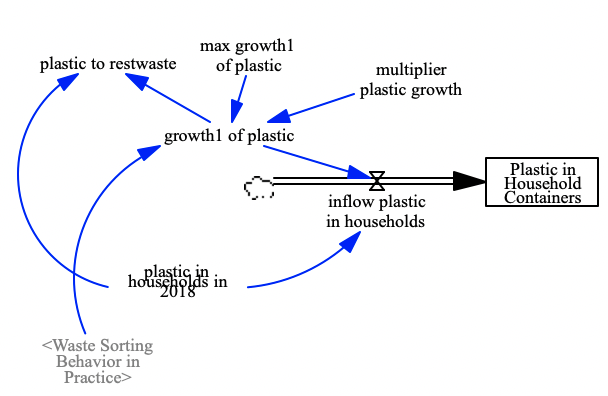
\includegraphics [scale=0.34,angle=360]{figures/plasticinflow.png}
\caption{Plastic in Households}
\label{fig:plasticinflow}
\end{figure}

\indent \newline
The variable "inflow plastic in households" is an inflow because it measures the rate of change in plastic in household containers. The equation computes the tons of plastic per year the household throws in the garbage and is affected by "growth1" in plastic and "plastic in household 2018".

\subsection{Growth1 of Plastic}

\indent \newline
The endogenous variable  "growth1 of plastic" is modeled as a minimum function that estimates the smallest values between the exogenous variable "max growth1 of plastic" and the stock "waste sorting behavior in practice", multiplied with the exogenous variable "multiplier plastic growth". The function gives an indication of how great the citizens are at sorting plastic. The minimum function also prevents the function from going negative. 

\subsection{Plastic to Rest Waste}

\indent \newline
The endogenous variable "plastic to rest waste" indicates the amount of plastic that is going into the rest waste. The equation takes the amount of plastic in households 2018 and multiplies it with 1 - growth1 of plastic. "Growth1 of plastic" suggests to what extent the citizens are sorting plastic. An increase in the value of the growth1 variable indicates that they are improving at sorting plastic. 

\subsection{Growth2 of Plastic}

\begin{figure}[H]
\centering
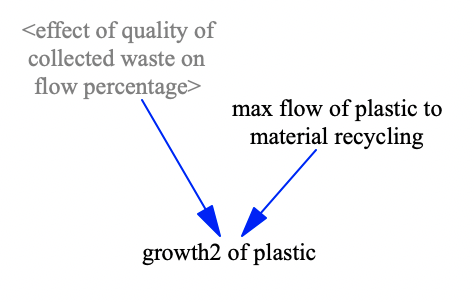
\includegraphics [scale=0.34,angle=360]{figures/plasticgrowth.png}
\caption{Growth2 of Plastic}
\label{fig:plasticgrowth}
\end{figure}

\indent \newline
"Growth2 of plastic" is formulated as an endogenous variable. The variable's equation is a minimum function, which calculates the smallest value of "max flow of plastic to material recycling" or "0.59 * effect of quality of collected waste on flow percentage". The minimum function also helps prevent the function from going negative.



